% !TEX root = ../agglo_clust_review.tex

\begin{figure}
\centering
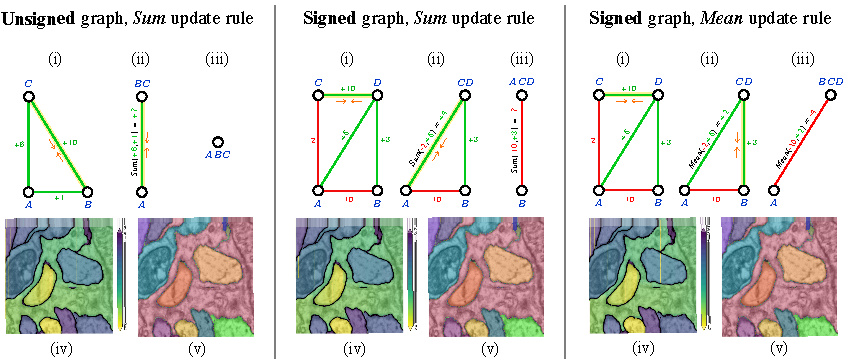
\includegraphics[width=0.50\textwidth,trim=0.4in 1.2in 0.in 0.05in,clip]{./figs/intro_image.pdf} % left bottom right top
\caption{\small 
Intro image: explain algorithm, main ideas and contributions \TODO{update colormap with a binary one. Atm it could look like another segmentation}
\label{fig:intro_figure}}
\end{figure}


\section{Introduction}
%On possible selling story could be: currently many of the successful proposal-free instance segmentation methods rely on a final clustering step on a grid-graph with both short and long-range connections. So it is worth to study this problem in more details. 


\begin{itemize}
\item \textbf{General intro about CNN:} big success in pixel-level image understanding tasks: boundary detection \cite{arbelaez2011contour,xie2015holistically,maninis2018convolutional}, semantic segmentation \cite{long2015fully,chen2018deeplab,kong2018recurrent}, optical flow \cite{weinzaepfel2013deepflow,dosovitskiy2015flownet}, pose estimation \cite{wei2016convolutional,cao2017realtime}...
% \SOURCE{\cite{kong2018recurrent}}
\item Many recent successful methods generate \textbf{region proposals} and classify the objects in the bounding box \cite{yang2012layered,ladicky2010and,hariharan2014simultaneous,chen2015multi,dai2016instance,liang2016reversible,he2017mask}
\item \emph{Why we do not like them}:
\begin{itemize}
\item rely on the object detector and non-maximum suppression heuristics to accurately “count” nb. of instances, 
\item underperform in cluttered scenes (assignment carried out independently for each detection) 
\item not usable for wiry or articulated segments/objects 
\item nothing in the architecture preventing a pixel to be shared between two instances
\item number of instances is limited by nb. proposals processed by CNN (usually hundreds). 
\item (difficult to train in an end-to-end manner: interface between instance segmentation and detection is non-differentiable)
% \item (architecture is complex and hard to tune and “debug”...?)
\end{itemize}

\item Among successful \textbf{proposal-free methods} there are: predict pixel embedding vectors \cite{kong2018recurrent,fathi2017semantic,newell2017associative,de2017semantic}; predict short- and long-range affinities \cite{liu2018affinity,wolf2018mutex,xie2015holistically} (more details in related work)

\item In both approaches we can obtain the final segmentation by using a \textbf{graph clustering algorithm}
\item Recent work (\cite{wolf2018mutex}, more...) shows that it is better to use \textbf{repulsion and attraction} (directly predict it with the classifier, no need to define seeds or to fix a threshold given an hierarchy of clusters)
\item solving correlation clustering problem (multicut) is too expensive for this application (even using recently proposed heuristics)
\item our contributions:
\begin{itemize}
\item we propose a unified and simple formalization of Agglomerative Clustering and show how many of the recently proposed methods can be seen as special cases (focusing in particular on signed graphs) (\textbf{review and comparison paper})
\item we propose several new clustering algorithms, among which one proved to be robust in our experiments (average linkage with must-not-link-edges)
\item we compare different types of agglomeration clustering on a pixel grid graph with short and long-range connections, focusing on aspects like efficieny, robustness (and MC energy) 

\end{itemize}
\item on other datasets (connectomics) many methods are based on multi-step pipelines first predicting superpixels
\item \textit{if we get good scores on CREMI}: we show that also on neuro-data it is worth to skip the hand-crafted superpixel step and compute the final segmentation directly from the CNN affinities (MWS already showed it on the ISBI dataset)

\end{itemize}
